\documentclass[pdf]{note}
\usepackage[usenames,dvipsnames]{color}     % for color coding during editing
\usepackage{verbatim}
\usepackage{url}
\usepackage[latin1]{inputenc}
\usepackage[T1]{fontenc}
\usepackage{ae}
\usepackage{amsmath, amssymb}
\usepackage{subfigure}
\usepackage{xspace}
\usepackage{multicol}
\usepackage{tabulary}

%\usepackage{finesse}
%\newcommand{\Finesse}{\textsc{Finesse}\xspace}

\usepackage{fancyvrb}
\DefineVerbatimEnvironment{finesse}{Verbatim}
{formatcom=\small}

\author{Charlotte Bond}
\shorttitle{OOMAO simulations with Fourier reconstructors}
\title{Simulations of adaptive optics systems using Fourier wavefront reconstructors in OOMAO}
\date{\today}
\issue{1}

%\usepackage{float}
%\usepackage{parskip}
%\usepackage{xspace}
\usepackage[pdftex,a4paper,pagebackref=true,pdfpagelabels=true]{hyperref}
\definecolor{linkcolor}{rgb}{.8,0,0}
\definecolor{urlcolor}{rgb}{0,0,.7}
\definecolor{citecolor}{rgb}{0,.5,0}
\definecolor{acrocolor}{rgb}{0,0,.7}
\hypersetup{bookmarksopen,colorlinks=true}
\hypersetup{pdfstartview=FitH}
\hypersetup{linktocpage=true,bookmarksnumbered=true}
\hypersetup{plainpages=false,breaklinks=true}
\hypersetup{linkcolor=linkcolor,citecolor=citecolor,urlcolor=urlcolor}

\DeclareMathOperator{\sinc}{sinc}

\newcommand{\tcr}{\textcolor{red}}

\let \IG \includegraphics

\begin{document}
\maketitle
\tableofcontents
\vspace{1cm}\hrule \vspace{1cm}

\section{Introduction}

This note details simulations carried out using OOMAO (Object Oriented Matlab Adaptive Optics Toolbox)
which compare different reconstructor methods, specifically traditional methods with Fourier
reconstructors.  We present the results of a new Fourier reconstructor which takes into account
the affects of aliasing in the measurement process.

\section{Traditional reconstructors}

Least square and mmse.

Check results got with these reconstructors.

\subsection{Residual PSD}
These results with 35\% coupling for DM influence functions.
In any adaptive optics system there is a correctable bandwidth, above which we can longer
correct higher spatial frequencies.  
\begin{figure}[htdp]
    \centerline{
      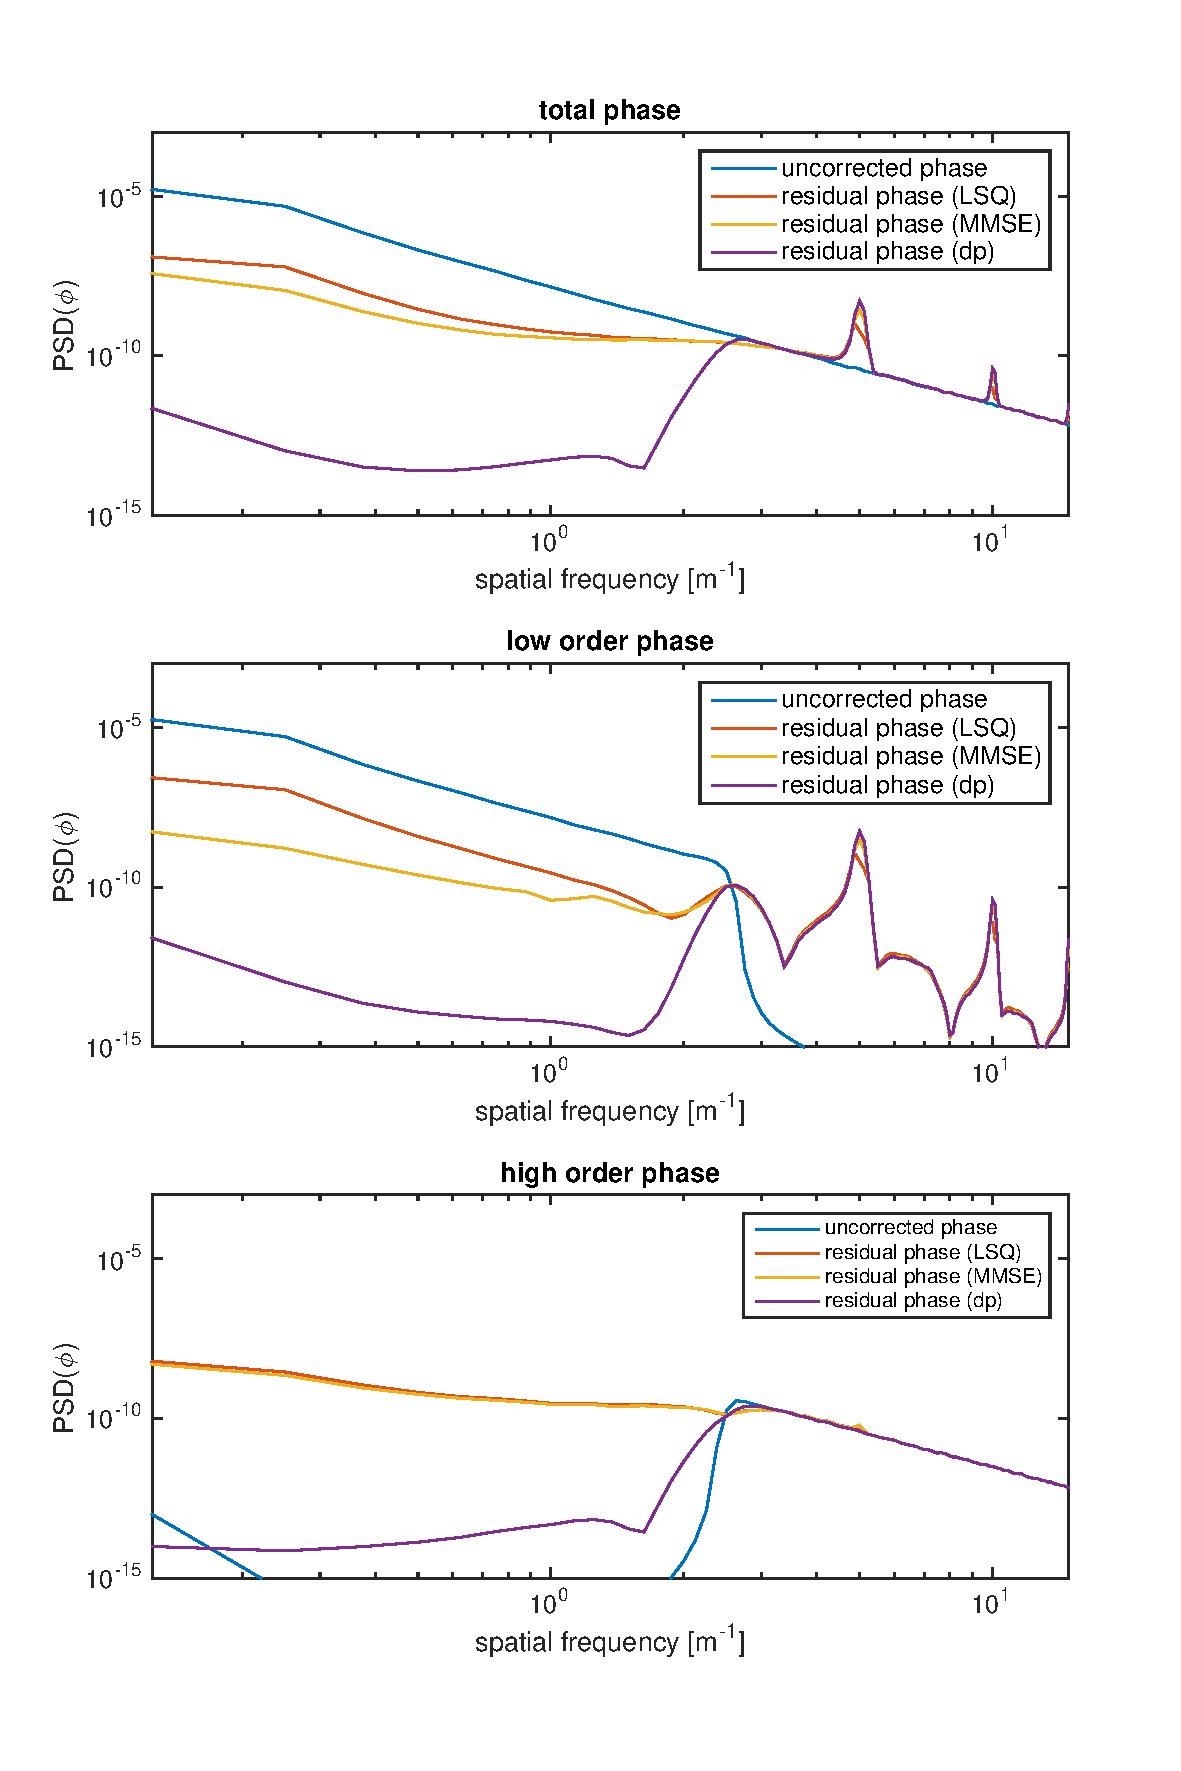
\includegraphics[trim = 10 40 10 40, clip, scale=0.7]{plots/residual_PSDs_from_different_phasecubes}
    }
    \caption{3 plots showing the power spectral density (PSD) of the residual phase after correction
    		with a deformable.  the 3 different plots correspond to 3 different phase screens.  From
		top to bottom we have: 1) total phase, including spatial frequencies within and outside
		the correctable band; 2) low order phase, with only spatial frequencies within the
		correctable band are included; and 3) high order phase, only spatial frequencies above
		the cut-off frequency are included.  For each phase screen we have 4 different phases:
		1) phase, the uncorrected phase; 2) LSQ, using a Least-Squares reconstruction method;
		3) MMSE, using a MMSE reconstruction method; and 4) DP, direct projection of the original
		phase on the deformable mirror modes.
    }
    \label{fig:PSDs_res_phase}
\end{figure}

\begin{figure}[htdp]
    \centerline{
      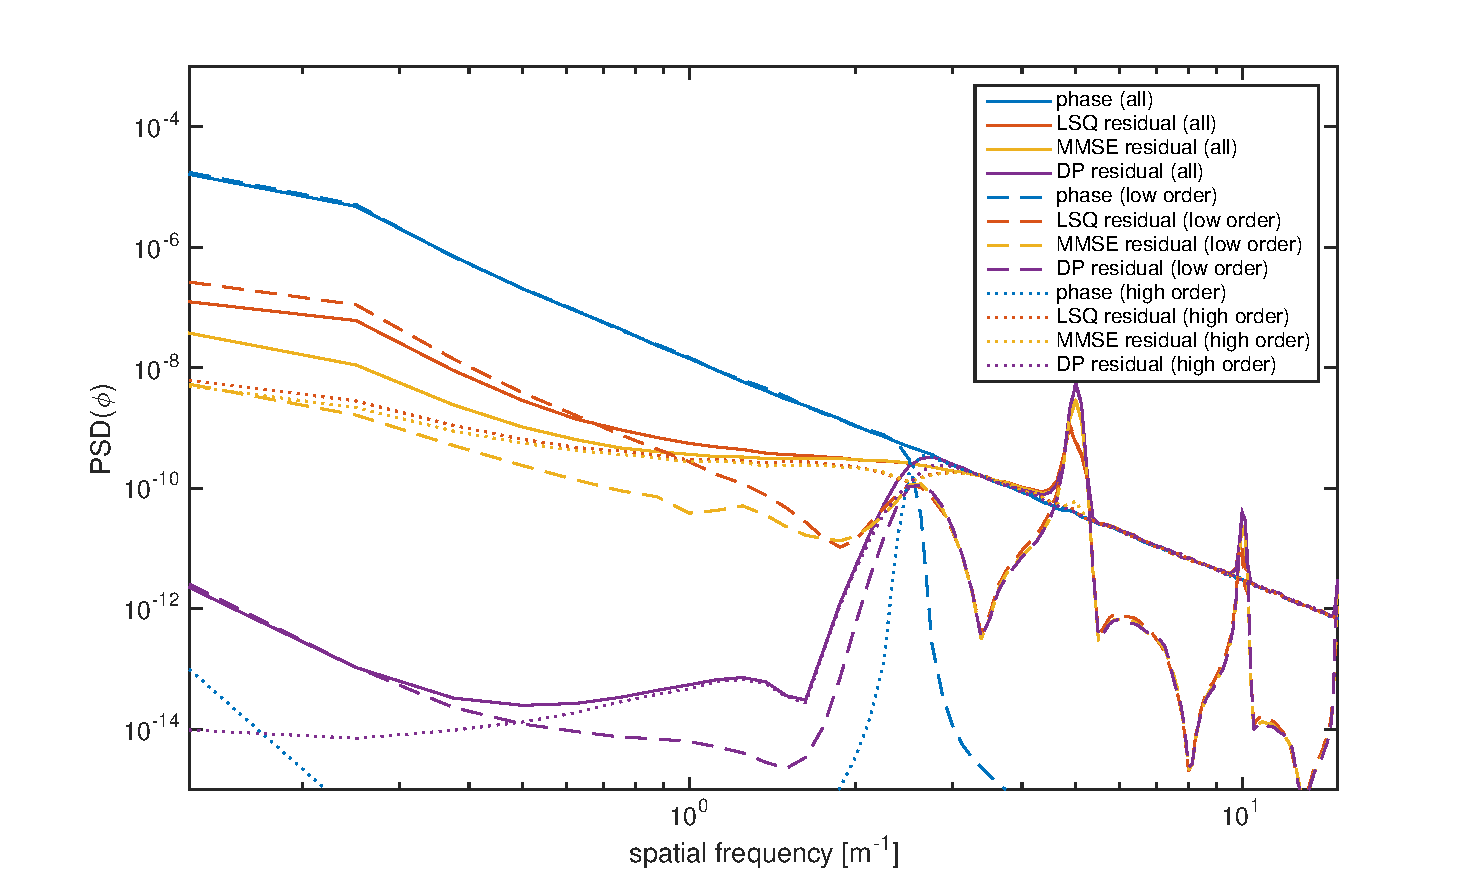
\includegraphics[scale=0.7]{plots/residual_PSDs}
    }
    \caption{PSD of residual phase for 3 phase screens: all spatial frequencies (all), in band spatial frequencies
    		(low order) and out of band spatial frequencies (high order).  For each phase screen type we have the
		PSD of the uncorrected phase and residual phases using 3 reconstructors: LSQ, MMSE and DP (direct projection).
    }
    \label{fig:res_PSDs}
\end{figure}

With plots showing all PSDs together we can identify where some of the features come from.

\begin{itemize}
\item Direct projection.  This shows us the minimum possible residual phase with this DM (i.e. we haven't
picked up any errors from the wavefront measurement process.  The total phase direct projection
is equivalent to the sum of the low order and high order parts.
\item The high order results show a significant increase in the PSD at low spatial frequencies (which shouldn't
be here as they are not in the original phase).  This suggests an limit to the accuracy of the wavefront
sensing or some noise, which means this level is the limit of our current AO setup.  In this case we would also
expect aliasing as we have high orders which will alias to lower orders.
\item The peaks in the data outside the band (at multiples of the actuator frequency) must come from
interaction with the DM.  The results suggest these peaks occur when we correct for low order terms (the
peaks don't appear in the high order phase screen residual).  When we are correcting these low order terms
we must be applying blind modes to the DM, which appear to excite these high frequencies.  
\end{itemize}

\newpage
\section{Fourier reconstruction: simple phase screen}

In this section I test the exact and anti-aliasing Fourier filters with a simple phase screen
with no aperture applied.  The simple phase screen only includes spatial frequencies which
are eigenmodes of the phase screen grid: for the given resolution and size.
The motivation for no aperture and a simple phase screen is to avoid having to use
the extra processing of extending the slopes out of the aperture and implementing
cyclic conditions on the slopes data.  This additional processing has the potential
to introduce additional errors, so we want to keep these first tests as simple as possible:
just testing the filters themselves.

\subsection{No deformable mirror}
To keep the first tests as simple as possible we don't include a deformable mirror (to
avoid any errors introduced by this process) and just deal purely with the phase.  The Fourier
reconstruction gives us the low resolution (reconstructed) phase, then using a Shannon interpolation we get
the high resolution phase which we compare with the original phase.

\subsubsection{Odd number of lenslets: no aliasing}

We start off with an odd number of lenslets, as there are issues with using an even number of
lenslets we will see later.

Firstly we look at the results (i.e. the power spectral density of the residual phase) for
a low order phase screen, to test the Fourier filters without the additional complication of
aliasing.  We will test 3 different filters, the original exact filter and two slight variations
on this filter.

\begin{table}[!h]
\begin{center}
\begin{tabular}{c|c|c}
filter		&	$R_x$					& $R_y$		\\
\hline
original	&	$K_x \sinc(d K_x) \sinc(dK_y) e^{i \pi d (K_x+K_y)}$
& $ K_y \sinc(d K_x) \sinc(dK_y) e^{i \pi d (K_x+K_y)}$ \\
new 1	&	$K_x \sinc(d_{g} K_x) \sinc(dK_y) e^{i \pi d (K_x+K_y)}$
& $ K_y \sinc(d K_x) \sinc(d_{g}K_y) e^{i \pi d (K_x+K_y)}$ \\
new 2 	& $K_x \sinc(d_g K_x) \sinc(dK_y) e^{i \pi d_g (K_x+K_y)}$
& $ K_y \sinc(d K_x) \sinc(d_gK_y) e^{i \pi d_g (K_x+K_y)}$ \\
\end{tabular}
\end{center}
\caption{3 different filters discussed in this note.  $K_x$ and $K_y$ refer to $x$ and $y$ spatial
		frequencies, $d$ is the lenslet spacing and $d_g$ is a modification to $d$ by
		the size of one pixel, as this is the distance across which the gradient is taken.}
\label{default}
\end{table}%

In figure~\ref{fig:PSDsPhase} several plots illustrating the PSD of residual phase are shown.
The top plot shows a slice through this PSD at $k_y = 0$.  There is some small improvement
in residual phase between the old method and the first new filter.  However, the real improvement
comes with filter new 2.  This is further illustrated by the full 2D PSDs shown in the two bottom plots.
On the left we have the results for the old filter, on the right for filter new 2. 
Again we see significant improvement using filter 2, although not as good as along the $k_x=0$ and
$k_y=0$ slices.  Currently I don't see any reason why we can not achieve as good in other areas,
as the $x$ and $y$ wavelengths are independent.  Are there still improvements/ alterations to the filters which could improve results in these areas?

\begin{figure}[htdp]
    \centerline{
      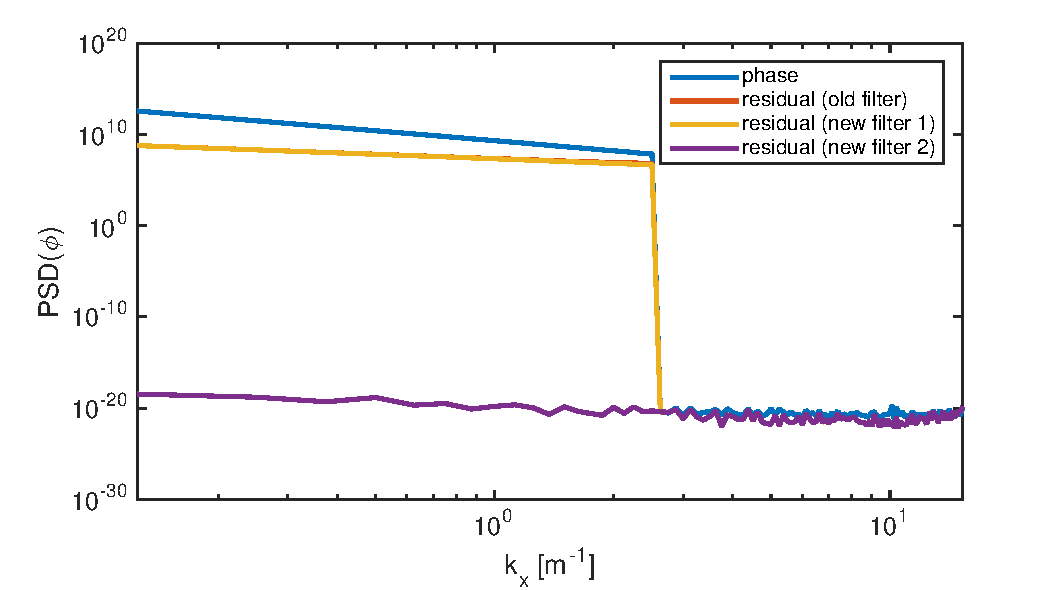
\includegraphics[scale=0.8]{plots/psdPhaseLO_Odd}
    }
    \centerline{
      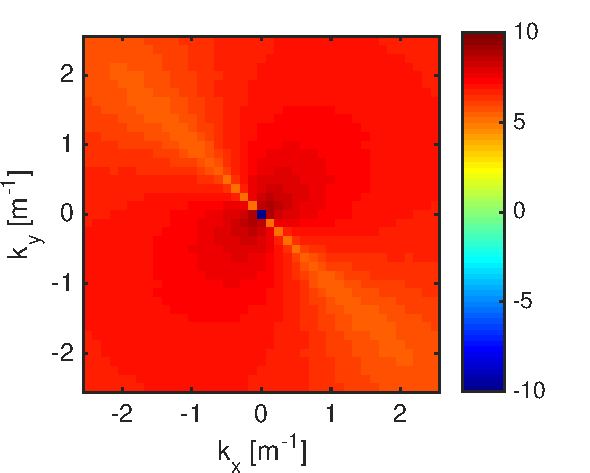
\includegraphics[scale=0.8]{plots/psdPhaseLO_Odd_2D_old}
      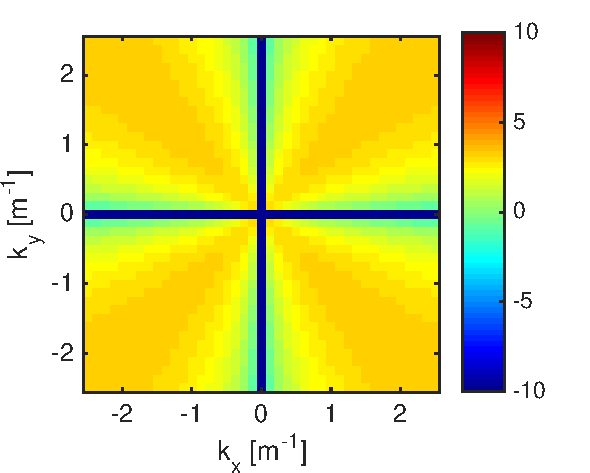
\includegraphics[scale=0.8]{plots/psdPhaseLO_Odd_2D_new2} 
    }
    \caption{Plots showing the power spectral density of the residual phase when different filters are
    		used.  {\bf Top:} PSD as a slice across $k_y = 0$ for the 3 filters, and also showing the
		PSD of the original non-corrected phase.  {\bf Bottom:}  log(PSD) of the residual phase for
		the original filter (left) and new 2 filter (right).  The new 2 filter is significantly better in terms
		of residual PSD, by at least 3-4 orders of magnitude across the frequency band.
    }
    \label{fig:PSDsPhase}
\end{figure}

In figure~\ref{fig:PSDsSlopes} the PSDs of the numeric and analytic $x$ slopes are compared.
These PSDs correspond to both new methods (1 and 2) as they differ by a phase which does
not affect the power spectral density.  In the top plot we see slices in $k_y$ of the PSD,
with the solid lines showing the theoretical values and the dashed lines showing the
numerical.  These match well.  In the bottom plot we see the fractional difference
for the whole 2D PSD.  We see slight differences across the PSD which will become smaller
and smaller as we average over a larger number of realisations of the generated phase screens.
As there is no discernible pattern in the residual it suggests the differences are merely a result
of the different random realisations.
For $k_x = 0$ the fractional difference is 1.  However, this is due to the theoretical value of 0, whilst
the numerical value is a negligible error ($\sim 10^{-33}$).


\begin{figure}[htdp]
    \centerline{
      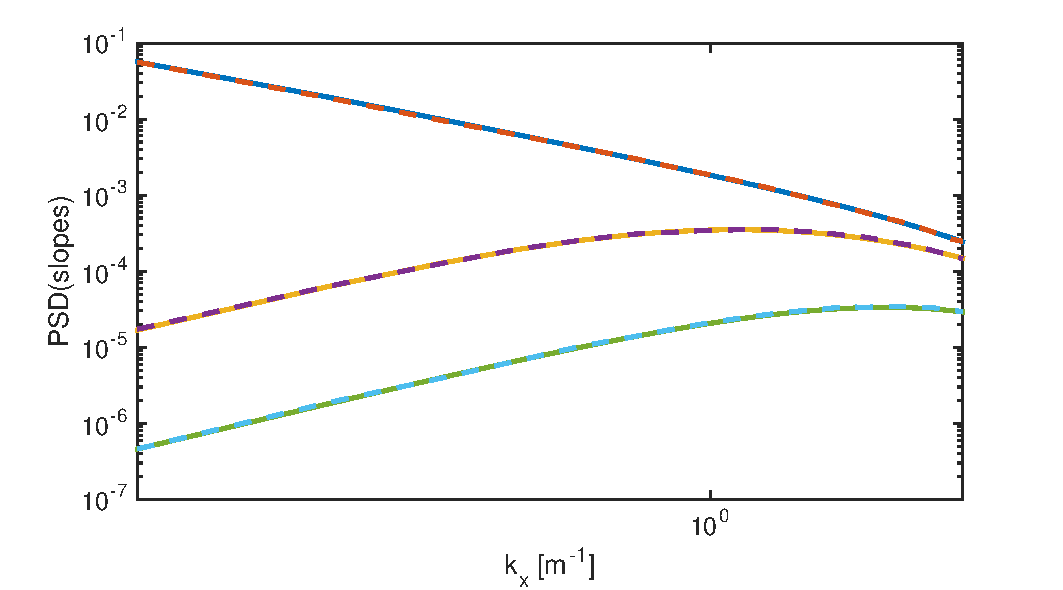
\includegraphics[scale=0.7]{plots/psdLOSlopesX_num_theory2_comp}
   }
    \centerline{   
      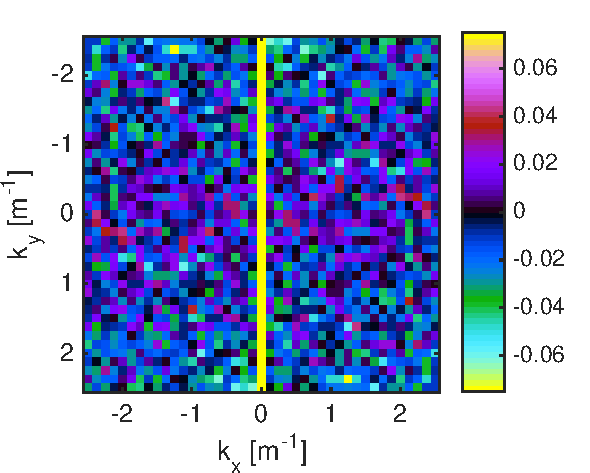
\includegraphics[scale=0.7]{plots/psdLOSlopesX_num_theory2_difference} 
    }
    \caption{Plots comparing the PSDs of the $x$ slopes from our numerical simulations
    		(with only low order terms, i.e. no aliasing)
    		and from theory (new methods 1 or 2, both give the same PSDs).  {\bf Top:}
		Plots showing the PSD vs $k_x$ for different slices in $k_y$.  The solid lines
		show the theoretical PSD, the dashed show the numerical result.
		{\bf Bottom:} Fractional difference between the numerical and theoretical
		results.  
    }
    \label{fig:PSDsSlopes}
\end{figure}

\newpage
\subsubsection{Odd number of lenslets: with aliasing}

Now we look at the results when we use a phase screen including orders higher
than those defined by the lenslet spacing, but still keeping a simple phase screen
(i.e. only spatial frequencies defined by the number of pixels and no aperture).  This
avoids the need for any windowing (i.e. Hanging window) to calculate the PSD.

Firstly we compare the PSD of the reconstructed phase for the total phase screen
(including all spatial frequencies) and a high order phase screen (including only
the spatial frequencies above the lenslet cut-off frequency), using the exact
filter.  If aliasing errors dominate
the residual we will expect the residuals of the total and high order phase screens
to match.  In each case the measurement process folds the high frequencies into the
correctable band and the system overcompensates for these correctable modes.
This is what we observe, as is seen in the simulation results shown in 
figure~\ref{fig:PSDPhaseTotal&HO}.

\begin{figure}[htdp]
    \centerline{
      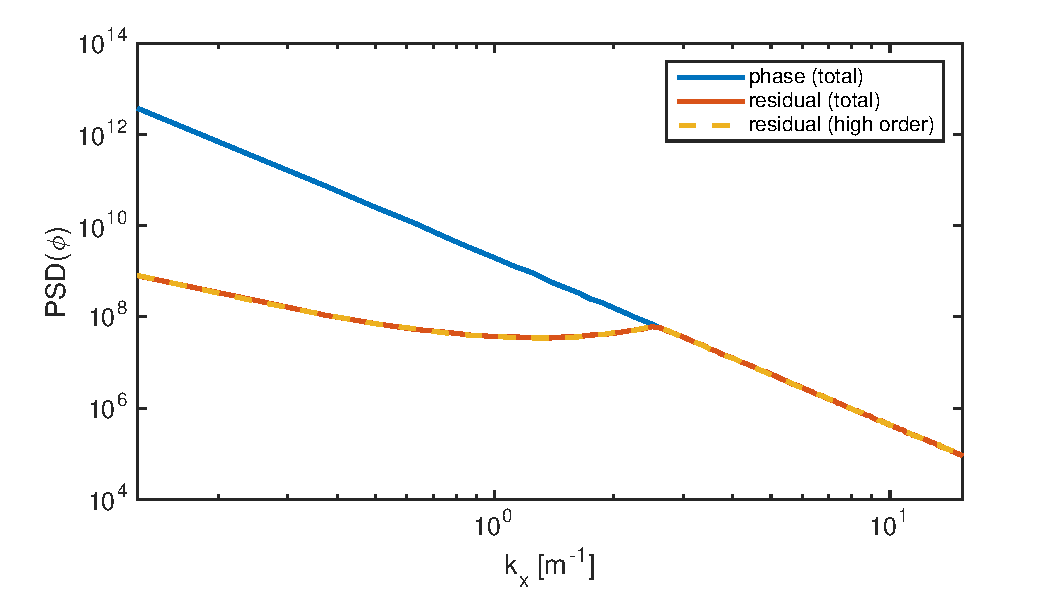
\includegraphics[scale=0.7]{plots/psdPhaseTotal&HO}
   }
    \caption{Plots of the PSD of the residual phase for the exact filter when a phase
    		screen including all spatial frequencies (total) is used and with only
		spatial frequencies above the lenslet cut-off (high order) is used.  The residuals
		are well matched, confirming that the aliasing of higher frequencies into the
		correction band is the dominant error.
    }
    \label{fig:PSDPhaseTotal&HO}
\end{figure}







\end{document}


